\section{Ammassi di galassie}\label{sec:ammassi-di-galassie}
In analogia con i gruppi, si riportano di seguito le caratteristiche che accomunano la maggior parte degli ammassi di galassie.

\noindent Il numero di galassie contenute è notevolmente maggiore al caso dei gruppi galattici, infatti contano circa $100$/$1000$ elementi. Le galassie contenute sono principalmente ellittiche e l’estensione radiale è compresa fra $1$ e $10$ $\si{Mpc}$.
La massa totale è di $10^{14}$--$10^{15}\, \si{\solarmass}$, mentre la dispersione di velocità è dell'ordine di $\SI{1000}{km.s^{-1}}$; si misurano dunque velocità maggiori rispetto a quelle dei gruppi.
Il rapporto massa--luce M/L varia in media da $100$ a $300$, valori molto simili a quelli che si misurano per i gruppi.

\noindent Una particolarità degli ammassi è che spesso, nel centro di essi, è presente una galassia molto massiccia e luminosa, detta “Brightest Cluster Galaxy” o “BCG” (si veda~\ref{sec:brightest-cluster-galaxy}).
Data l’elevata massa essi spesso fungono da lenti gravitazionali per altre galassie e \emph{QSO's} (Quasi-Stellar Objects) che si trovano dietro l’ammasso stesso.
Infine è importante notare che, nonostante gli ammassi siano formati principalmente da galassie, la materia galattica costituisce solo il $5\%$ della massa complessiva di essi, il gas caldo diffuso presente (cap.~\ref{sec:intra-cluster-medium}) ne costituisce il $15\%$, mentre il restante $80\%$ è opera della materia oscura.

%serie di immagini con ammassi a diverse bande elettromagnetiche

\subsection{Intra-Cluster Medium}\label{sec:intra-cluster-medium}
Il gas caldo diffuso precedentemente citato prende il nome di Intra--Cluster Medium o ICM. Esso possiede in media una massa di $10^{14}\, \si{\solarmass}$ ed emette una luminosità di $10^{43}$--$\SI{e46}{erg.s^{-1}}$ principalmente emessa sotto forma di raggi X come è prevedibile ricordando la legge di Wien
\begin{equation}
    \lambda = \frac{b}{T}                                         \qquad b \approx \num{2.9e-3} \si{m.K} 
\end{equation}
e inserendo come temperatura T$\sim 10^7$--$\SI{e8}{K}$.
Comparando le immagini~\ref{fig:visible-icm} e~\ref{fig:icm}, le quali raffigurano uno stesso ammasso rispettivamente nel visibile e in banda X, si noti come l'ICM sia visibile solo tramite osservazioni in banda X.
Sebbene possieda un’elevata temperatura, la bassa densità del gas non permette il bruciamento degli atomi di idrogeno e di elio ($\rho_{ICM}\sim 10^{-2}$-- $10^{-4}\:\si{atomi.cm^{-3}}$).
La metallicità dell’ICM è particolarmente elevata, è circa pari al $30\%$ di quella solare e questo indica al fatto che non si tratta di un gas primordiale, ma di un composto arricchito da precedenti fenomeni astrofisici.
\begin{figure}
    \centering
    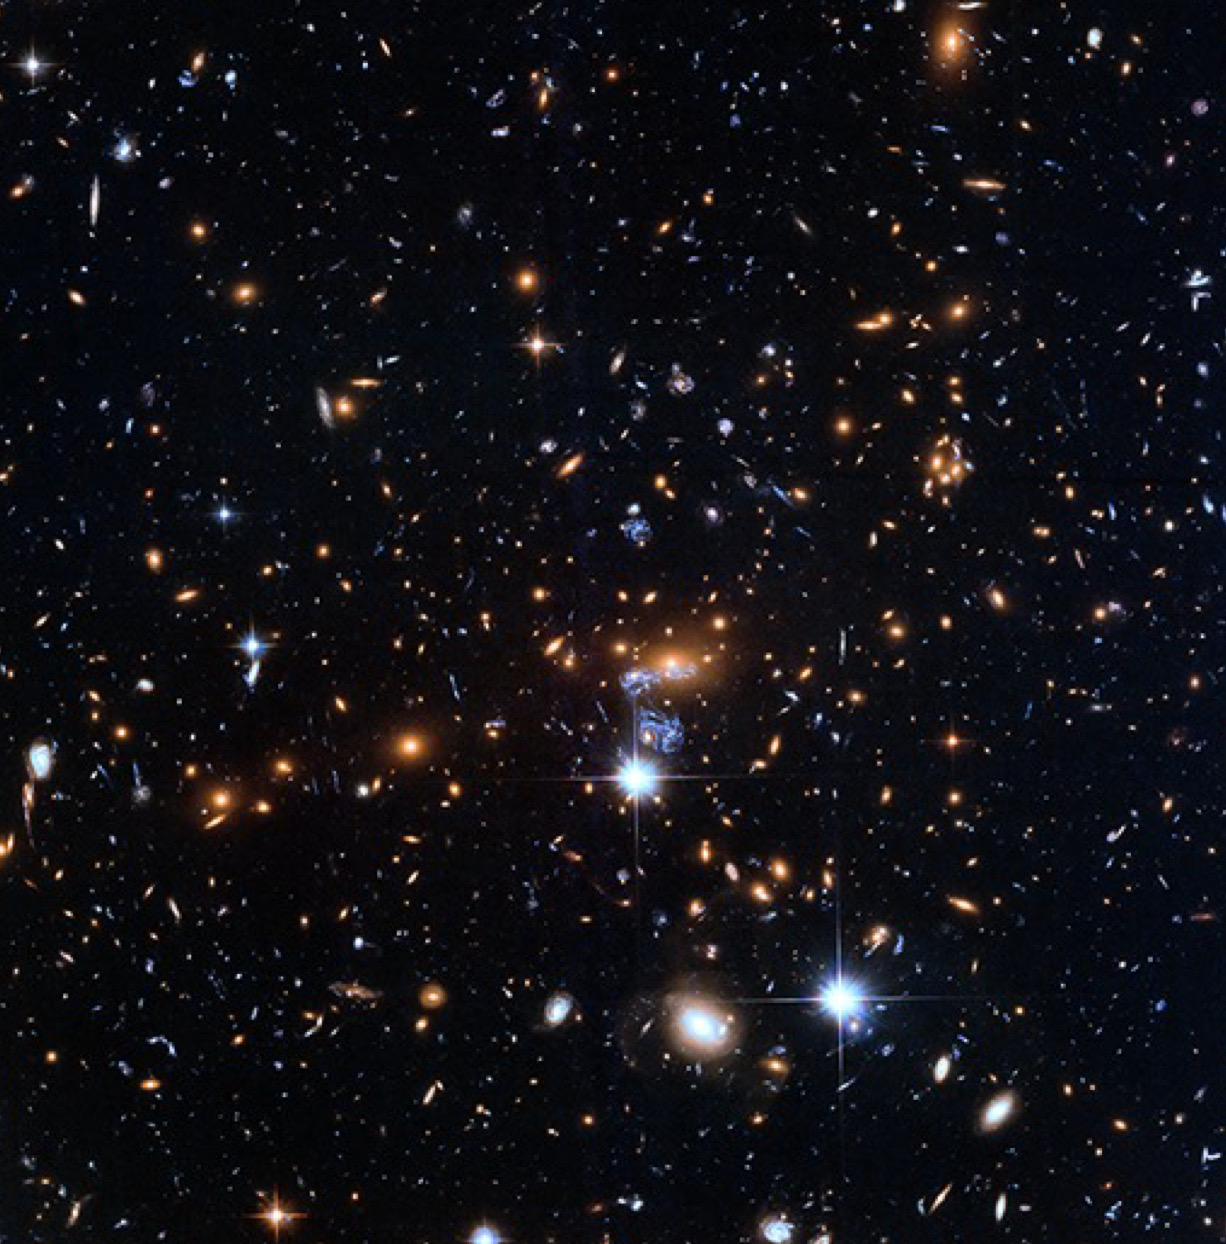
\includegraphics[width = 0.5\textwidth]{immagini/visible-icm.png}
    \caption{L'ammasso MACS J$1149.6+2223$ osservato nel visibile}
    \label{fig:visible-icm}
\end{figure}
\begin{figure}
    \centering
    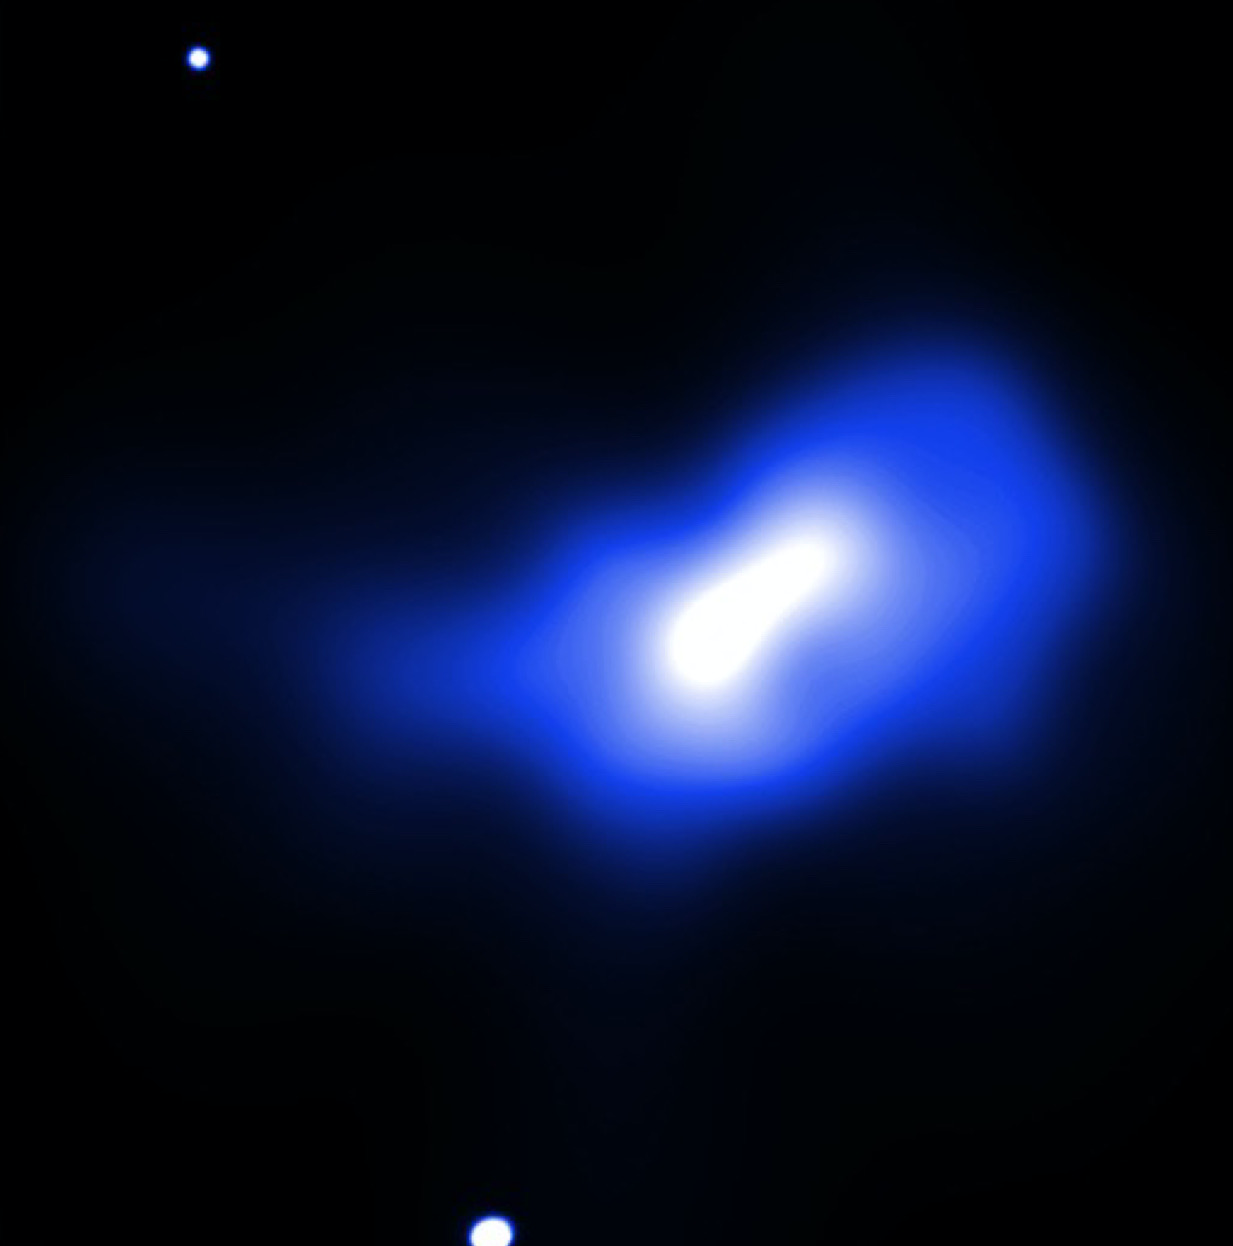
\includegraphics[width = 0.5\textwidth]{immagini/icm.png}
    \caption{L'ammasso MACS J$1149.6+2223$ osservato in banda X, in blu l'ICM}
    \label{fig:icm}
\end{figure}
Data l’elevata temperatura del gas gli atomi vengono quasi interamente ionizzati dando così vita ad uno stato di plasma molto caldo (si pensi che sono presenti atomi ionizzati Fe$^{25+}$).

\subsubsection{Radiazione di frenamento o Bremsstrahlung}\label{sec:bremsstrahlung}
Un fenomeno di notevole importanza che caratterizza l'ICM è l'emissione di radiazione tramite frenamento o \emph{bremsstrahlung}. 
Questo fenomeno si verifica in presenza di plasma caldo e viene descritto nel seguente modo: gli elettroni liberi, influenzati dal campo elettrico degli ioni del plasma, vengono decelerati, questo comporta una diminuzione della loro energia cinetica e l’emissione di fotoni, ovvero radiazione elettromagnetica.

\subsection{Stima della massa totale tramite ICM}
Lo studio dell’intra--cluster medium (ICM) ci permette di stimare la massa totale dell’ammasso di cui fa parte.
Bisogna fare delle ipotesi prima di procedere: 
si suppone che sia presente una simmetria sferica nell’ammasso e che l’ICM si trovi in uno stato di equilibrio idrostatico; non devono essere presenti né una variazione di temperatura, né un’espansione del gas.
Inoltre il gas viene ipotizzato ideale.

\noindent Partendo dall’equazione di equilibrio idrostatico in un potenziale sferico: 
\begin{equation} 
    \frac{dP}{dr} = - \frac{GM(r)}{r^2} \rho(r) 
\end{equation}
si ricava:
\begin{equation}\label{eq:equilibrio-idrostatico-2}
M(r) = - \frac{r^2}{G \rho(r)} \frac{dP}{dr}
\end{equation}
Ricordando l'espressione della pressione per gas ideale
\begin{equation} \label{eq:pressione-gas-ideale}
    P = \frac{k\rho T}{\mu H} \implies \frac{dP}{dr} = \frac{k}{\mu H}\Bigl[ T\frac{d\rho}{dr}+\rho \frac{dT}{dr}\Bigr]
\end{equation}
e sostituendo la~\refeq{eq:pressione-gas-ideale} nella~\refeq{eq:equilibrio-idrostatico-2} si ottiene:
\begin{equation}
    M(r) = \frac{k\,r\,T}{G\,\mu\,H}\Bigl[-\frac{d\:\ln{\rho(r)}}{d\:\ln{r}} - \frac{d\:\ln{T(r)}}{d\:\ln{r}}\Bigr]
\end{equation}

Quindi dalla misurazione dei profili di temperatura $T(r)$ e di densità $\rho(r)$ del gas (ottenibili dagli spettri di raggi X) si può stimare la massa totale $M$. 

\noindent N.B. è lo stesso metodo che viene utilizzato con le galassie ellittiche (REFERENZA), anch’esse forti emettitrici di raggi X.

Questo metodo indiretto di misurazione della massa presenta sia dei vantaggi sia degli svantaggi rispetto a metodi alternativi.

\subsubsection{\textbf{Vantaggi:}} 
\begin{itemize}
    \item Se si volesse stimare la massa tramite uno studio cinematico con l'utilizzo del teorema del viriale (vedi eq.~\refeq{eq:teorema-viriale}), si dovrebbe richiedere l'isotropia della distribuzione delle velocità dell'ammasso. Tale richiesta non viene soddisfatta in molti casi. 
    \item La massa potrebbe essere stimata tramite il fenomeno di lente gravitazionale (fig.~\ref{fig:lensing}): tale metodo è però svantaggioso in quanto affinché tale effetto sia misurabile si ha bisogno della presenza di altri oggetti astronomici sullo sfondo dell’ammasso, non sempre disponibili.
\end{itemize} 

\begin{figure}
    \centering
    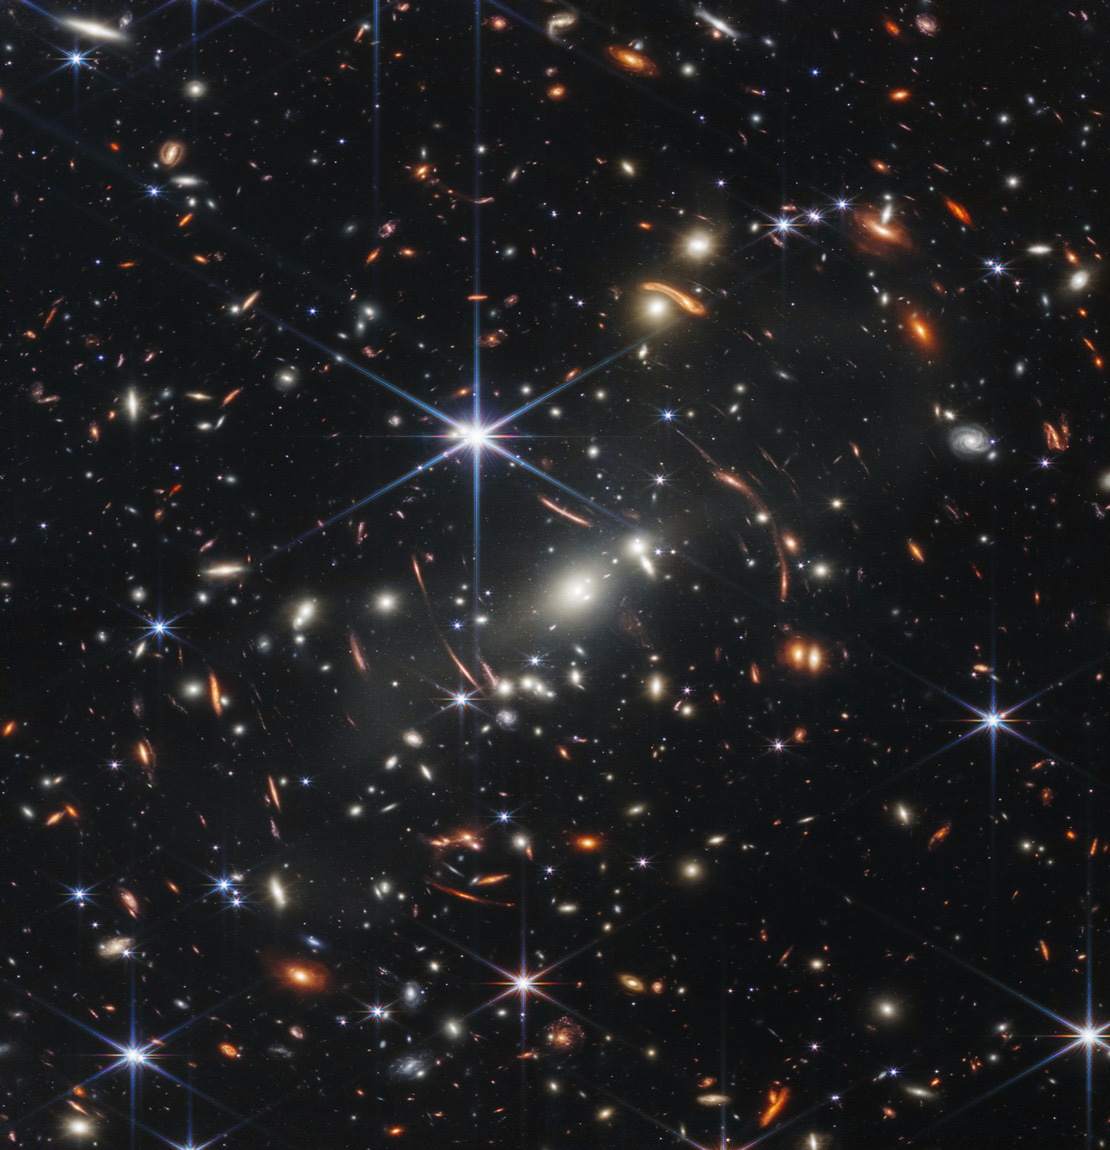
\includegraphics[width = 0.5\textwidth]{immagini/lensing.png}
    \caption{Nell'immagine sono ben visibili i fenomeni di deformazione gravitazionale}
    \label{fig:lensing}
\end{figure}

\subsubsection{\textbf{Svantaggi:}} 
\begin{itemize}
    \item Determinare i valori di $\rho(r)$ e $T(r)$ tramite la radiazione ricevuta non è sempre fattibile, in quanto, con l’aumentare della distanza, il segnale ricevuto risulta sempre più debole. 
    \item L’ipotesi di simmetria sferica risulta valida solo per ammassi \emph{well relaxed} (un esempio in figura~\ref{fig:well-relaxed-cluster}), ovvero quegli ammassi non sottoposti a rilevanti squilibri dinamici e termici, e dove lo spettro di radiazione è regolare (è richiesto un ICM in equilibrio idrostatico).
\end{itemize}
\begin{figure}
    \centering
    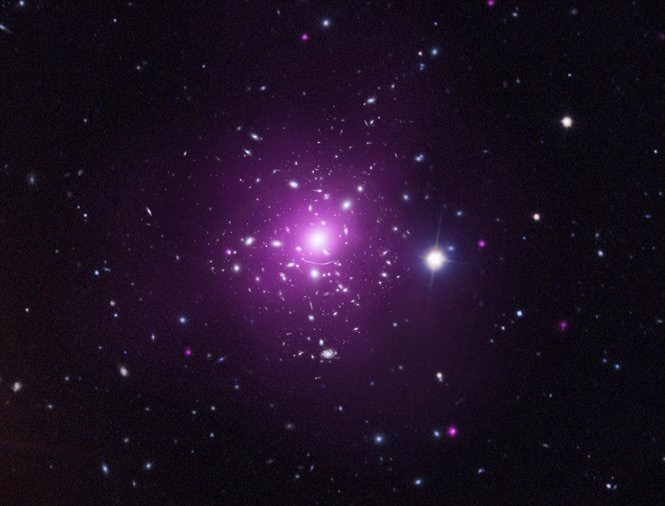
\includegraphics[width = 0.5\textwidth]{immagini/relaxed-cluster.png}
    \caption{Immagine di Abell 383, un esempio di ammasso well-relaxed}
    \label{fig:well-relaxed-cluster}
\end{figure}
